\documentclass{ximera}

\title{Practice for Eigenvalue Method}

%\auor{Matthew Charnley and Jason Nowell}
\usepackage[margin=1.5cm]{geometry}
\usepackage{indentfirst}
\usepackage{sagetex}
\usepackage{lipsum}
\usepackage{amsmath}
\usepackage{mathrsfs}


%%% Random packages added without verifying what they are really doing - just to get initial compile to work.
\usepackage{tcolorbox}
\usepackage{hypcap}
\usepackage{booktabs}%% To get \toprule,\midrule,\bottomrule etc.
\usepackage{nicefrac}
\usepackage{caption}
\usepackage{units}

% This is my modified wrapfig that doesn't use intextsep
\usepackage{mywrapfig}
\usepackage{import}



%%% End to random added packages.


\graphicspath{
    {./figures/}
    {./../figures/}
    {./../../figures/}
}
\renewcommand{\log}{\ln}%%%%
\DeclareMathOperator{\arcsec}{arcsec}
%% New commands


%%%%%%%%%%%%%%%%%%%%
% New Conditionals %
%%%%%%%%%%%%%%%%%%%%


% referencing
\makeatletter
    \DeclareRobustCommand{\myvref}[2]{%
      \leavevmode%
      \begingroup
        \let\T@pageref\@pagerefstar
        \hyperref[{#2}]{%
	  #1~\ref*{#2}%
        }%
        \vpageref[\unskip]{#2}%
      \endgroup
    }%

    \DeclareRobustCommand{\myref}[2]{%
      \leavevmode%
      \begingroup
        \let\T@pageref\@pagerefstar
        \hyperref[{#2}]{%
	  #1~\ref*{#2}%
        }%
      \endgroup
    }%
\makeatother

\newcommand{\figurevref}[1]{\myvref{Figure}{#1}}
\newcommand{\figureref}[1]{\myref{Figure}{#1}}
\newcommand{\tablevref}[1]{\myvref{Table}{#1}}
\newcommand{\tableref}[1]{\myref{Table}{#1}}
\newcommand{\chapterref}[1]{\myref{chapter}{#1}}
\newcommand{\Chapterref}[1]{\myref{Chapter}{#1}}
\newcommand{\appendixref}[1]{\myref{appendix}{#1}}
\newcommand{\Appendixref}[1]{\myref{Appendix}{#1}}
\newcommand{\sectionref}[1]{\myref{\S}{#1}}
\newcommand{\subsectionref}[1]{\myref{subsection}{#1}}
\newcommand{\subsectionvref}[1]{\myvref{subsection}{#1}}
\newcommand{\exercisevref}[1]{\myvref{Exercise}{#1}}
\newcommand{\exerciseref}[1]{\myref{Exercise}{#1}}
\newcommand{\examplevref}[1]{\myvref{Example}{#1}}
\newcommand{\exampleref}[1]{\myref{Example}{#1}}
\newcommand{\thmvref}[1]{\myvref{Theorem}{#1}}
\newcommand{\thmref}[1]{\myref{Theorem}{#1}}


\renewcommand{\exampleref}[1]{ {\color{red} \bfseries Normally a reference to a previous example goes here.}}
\renewcommand{\figurevref}[1]{ {\color{red} \bfseries Normally a reference to a previous figure goes here.}}
\renewcommand{\tablevref}[1]{ {\color{red} \bfseries Normally a reference to a previous table goes here.}}
\renewcommand{\Appendixref}[1]{ {\color{red} \bfseries Normally a reference to an Appendix goes here.}}
\renewcommand{\exercisevref}[1]{ {\color{red} \bfseries Normally a reference to a previous exercise goes here.}}



\newcommand{\R}{\mathbb{R}}

%% Example Solution Env.
\def\beginSolclaim{\par\addvspace{\medskipamount}\noindent\hbox{\bf Solution:}\hspace{0.5em}\ignorespaces}
\def\endSolclaim{\par\addvspace{-1em}\hfill\rule{1em}{0.4pt}\hspace{-0.4pt}\rule{0.4pt}{1em}\par\addvspace{\medskipamount}}
\newenvironment{exampleSol}[1][]{\beginSolclaim}{\endSolclaim}

%% General figure formating from original book.
\newcommand{\mybeginframe}{%
\begin{tcolorbox}[colback=white,colframe=lightgray,left=5pt,right=5pt]%
}
\newcommand{\myendframe}{%
\end{tcolorbox}%
}

%%% Eventually return and fix this to make matlab code work correctly.
%% Define the matlab environment as another code environment
%\newenvironment{matlab}
%{% Begin Environment Code
%{ \centering \bfseries Matlab Code }
%\begin{code}
%}% End of Begin Environment Code
%{% Start of End Environment Code
%\end{code}
%}% End of End Environment Code


% this one should have a caption, first argument is the size
\newenvironment{mywrapfig}[2][]{
 \wrapfigure[#1]{r}{#2}
 \mybeginframe
 \centering
}{%
 \myendframe
 \endwrapfigure
}

% this one has no caption, first argument is size,
% the second argument is a larger size used for HTML (ignored by latex)
\newenvironment{mywrapfigsimp}[3][]{%
 \wrapfigure[#1]{r}{#2}%
 \centering%
}{%
 \endwrapfigure%
}
\newenvironment{myfig}
    {%
    \begin{figure}[h!t]
        \mybeginframe%
        \centering%
    }
    {%
        \myendframe
    \end{figure}%
    }


% graphics include
\newcommand{\diffyincludegraphics}[3]{\includegraphics[#1]{#3}}
\newcommand{\myincludegraphics}[3]{\includegraphics[#1]{#3}}
\newcommand{\inputpdft}[1]{\subimport*{../figures/}{#1.pdf_t}}


%% Not sure what these even do? They don't seem to actually work... fun!
%\newcommand{\mybxbg}[1]{\tcboxmath[colback=white,colframe=black,boxrule=0.5pt,top=1.5pt,bottom=1.5pt]{#1}}
%\newcommand{\mybxsm}[1]{\tcboxmath[colback=white,colframe=black,boxrule=0.5pt,left=0pt,right=0pt,top=0pt,bottom=0pt]{#1}}
\newcommand{\mybxsm}[1]{#1}
\newcommand{\mybxbg}[1]{#1}

%%% Something about tasks for practice/hw?
\usepackage{tasks}
\usepackage{footnote}
\makesavenoteenv{tasks}


%% For pdf only?
\newcommand{\diffypdfversion}[1]{#1}


%% Kill ``cite'' and go back later to fix it.
\renewcommand{\cite}[1]{}


%% Currently we can't really use index or its derivatives. So we are gonna kill them off.
\renewcommand{\index}[1]{}
\newcommand{\myindex}[1]{#1}







\begin{document}
\begin{abstract}
Why?
\end{abstract}
\maketitle


\begin{exercise}
    \begin{itemize}
        \item Find the general solution of $x_1' = 2 x_1$, $x_2' = 3 x_2$ using the eigenvalue method (first write the system in the form ${\vec{x}}' = A \vec{x}$).
        \item Solve the system by solving each equation separately and verify you get the same general solution.
    \end{itemize}
    $C_1\left[\begin{smallmatrix} \answer{1} \\ 0 \end{smallmatrix}\right]e^{2t} + C_2\left[\begin{smallmatrix} 0 \\ \answer{1}  \end{smallmatrix}\right]e^{3t}$
\end{exercise}
%\comboSol
%{%
%$C_1\left[\begin{smallmatrix} 1 \\ 0 \end{smallmatrix}\right]e^{2t} + C_2\left[\begin{smallmatrix} 0 \\ 1  \end{smallmatrix}\right]e^{3t}$
%}

\begin{exercise}
    Find the general solution of $x_1' = 3 x_1 + x_2$, $x_2' = 2 x_1 + 4 x_2$ using the eigenvalue method and sketch the phase portrait for this system of differential equations.\\
    $C_1 \left[\begin{smallmatrix} \answer{1} \\ -1 \end{smallmatrix}\right]e^{2t} + C_2\left[\begin{smallmatrix} 1 \\ \answer{2} \end{smallmatrix}\right]e^{-t}$
\end{exercise}
%\comboSol
%{%
%$C_1 \left[\begin{smallmatrix} 1 \\ -1 \end{smallmatrix}\right]e^{2t} + C_2\left[\begin{smallmatrix} 1 \\ 2 \end{smallmatrix}\right]e^{-t}$ \hfill
%\raisebox{-0.5\height}{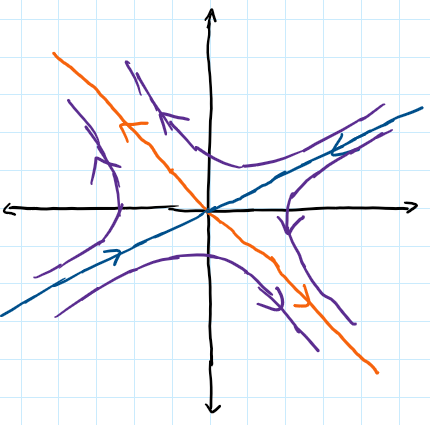
\includegraphics[height=1.5in]{Images/phaseportrait_3_1_2_4_sketch.png}} \hfill \hfill
%}

\begin{exercise}%
    Solve $x_1' = x_2$, $x_2' = x_1$ using the eigenvalue method and sketch the phase portrait for this system of differential equations.\\
    $\vec{x} = C_1 \left[ \begin{smallmatrix}
        \answer{1} \\ 1
    \end{smallmatrix}\right] e^{t}
    + C_2 
    \left[ \begin{smallmatrix}
        1 \\ \answer{-1}
    \end{smallmatrix}\right] e^{-t}$
\end{exercise}
%\exsol{%
%$\vec{x} = C_1 \left[ \begin{smallmatrix}
%1 \\ 1
%\end{smallmatrix}\right] e^{t}
%+
%C_2 \left[ \begin{smallmatrix}
%1 \\ -1
%\end{smallmatrix}\right] e^{-t}$ \hfill
%\raisebox{-0.5\height}{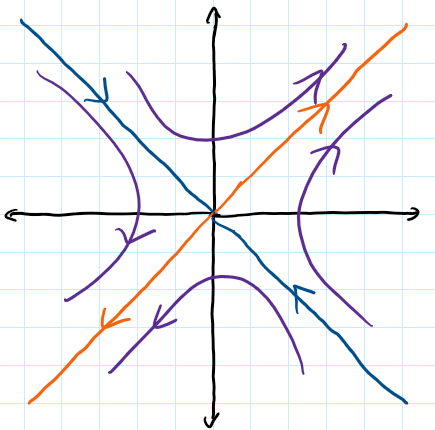
\includegraphics[height=1.5in]{Images/phaseportrait_0_1_1_0_sketch.png}} \hfill\hfill
%}


\begin{exercise}
    Amino acid dating can be used by forensic scientists to determine the time of death in situations where other techniques might not work. These amino acids are sneaky, and they exist in a left-handed form (L) and a right-handed form (D), which are called {\it enantiomers}. While you’re alive, your body keeps all your amino acids in the L form. Once you die, your body no longer regulates your amino acids, and every so often they flip a coin and decide whether to switch into the opposite form. This way, when someone finds your body in a dumpster, they can pull out your teeth and measure the {\it racemization ratio}, which is the ratio of D-enantiomers to L-enantiomers. %4.4

    Denote by $D(t)$ and $L(t)$, respectively, the proportions of D- and L-enantiomers found in your teeth, where $t$ is measured in years after death. Since this is Math class, the proportions are governed by a system of differential equations, such as
    \begin{equation}
        \begin{bmatrix} 
            L' \\ 
            D' 
        \end{bmatrix} 
        = 
        \begin{bmatrix} 
            -.02& .02\\ 
            .02 & -.02 
        \end{bmatrix}
        \begin{bmatrix} 
            L\\ 
            D 
        \end{bmatrix}.\label{eq:AminoEqn}
    \end{equation}
    \begin{itemize}
        \item Find the general solution to \eqref{eq:AminoEqn}.\\
            $\vec{x}(t) = C_1 \left[\begin{smallmatrix} \answer{-1} \\ 1 \end{smallmatrix}\right]e^{-t/25} + C_2\left[\begin{smallmatrix} 1 \\ \answer{1} \end{smallmatrix}\right]$
        \item Solve \eqref{eq:AminoEqn} with initial conditions $D(0) = 0$ and $L(0) = 1$, and express the solution in component form. Describe what happens to the quantities $D(t)$ and $L(t)$ in the long run.\\
            $L(t) = \answer{\frac{1}{2} + \frac{1}{2}e^{-\frac{t}{25}}}$, $D(t) = \answer{\frac{1}{2} - \frac{1}{2}e^{-\frac{t}{25}}}$
        \item Given the above initial conditions, if the racemization ratio in your teeth is currently 1:3, how long ago did you die?  $t = \answer{25\ln(2)}$  years
    \end{itemize}
\end{exercise}
%\comboSol
%{%
%a)~ $\vec{x}(t) = C_1 \left[\begin{smallmatrix} -1 \\ 1 \end{smallmatrix}\right]e^{-t/25} + C_2\left[\begin{smallmatrix} 1 \\ 1 \end{smallmatrix}\right]$ \\ b)~ $L(t) = \frac{1}{2} + \frac{1}{2}e^{-t/25},\ D(t) = \frac{1}{2} - \frac{1}{2}e^{-t/25}$. Both go to $1/2$. \\ c)~ $t = 25\ln(2)\approx 17.33$ years
%}

\begin{exercise}
    \begin{itemize}
        \item Compute eigenvalues and eigenvectors of
        $A = 
        \left[ 
            \begin{smallmatrix}
                9 & -2 & -6 \\
                -8 & 3 & 6 \\
                10 & -2 & -6
            \end{smallmatrix} 
        \right]$.\\
            $\lambda_1 = \answer{1}$, $\vec{v}_1 = \left[\begin{smallmatrix} \answer{\frac{1}{2}} \\ -1 \\ \answer{1} \end{smallmatrix}\right]$. $\lambda_2 = \answer{2}$, $\vec{v}_2 = \left[\begin{smallmatrix} 2 \\ \answer{-2} \\ \answer{3} \end{smallmatrix}\right]$. $\lambda_3 = \answer{3}$, $\vec{v}_3 = \left[\begin{smallmatrix} \answer{3} \\ -3 \\ \answer{4} \end{smallmatrix}\right]$
        \item Find the general solution of ${\vec{x}}' = A \vec{x}$.\\
            $\vec{x}(t) = C_1\left[\begin{smallmatrix} \answer{\frac{1}{2}} \\ -1 \\ \answer{1} \end{smallmatrix}\right]e^t + C_2\left[\begin{smallmatrix} \answer{2} \\ \answer{-2} \\ 3 \end{smallmatrix}\right]e^{2t} + C_3\left[\begin{smallmatrix} \answer{3} \\ -3 \\ \answer{4} \end{smallmatrix}\right]e^{3t}$
    \end{itemize}
\end{exercise}
%\comboSol
%{%
%a)~ $\lambda_1 = 1$, $\vec{v}_1 = \left[\begin{smallmatrix} 1/2 \\ -1 \\ 1 \end{smallmatrix}\right]$. $\lambda_2 = 2$, $\vec{v}_2 = \left[\begin{smallmatrix} 2 \\ -2 \\ 3 \end{smallmatrix}\right]$. $\lambda_3 = 3$, $\vec{v}_3 = \left[\begin{smallmatrix} 3 \\ -3 \\ 4 \end{smallmatrix}\right]$ \\
%b)~ $\vec{x}(t) = C_1\left[\begin{smallmatrix} 1/2 \\ -1 \\ 1 \end{smallmatrix}\right]e^t + C_2\left[\begin{smallmatrix} 2 \\ -2 \\ 3 \end{smallmatrix}\right]e^{2t} + C_3\left[\begin{smallmatrix} 3 \\ -3 \\ 4 \end{smallmatrix}\right]e^{3t}$
%}

\begin{exercise}%
    \begin{itemize}
        \item Compute eigenvalues and eigenvectors of
            $A= 
            \left[ 
                \begin{smallmatrix}
                    1 & 0 & 3 \\
                    -1 & 0 & 1 \\
                    2 & 0 & 2
                \end{smallmatrix}
            \right]$.\\
            Eigenvalues: $\answer{-1}$, $\answer{0}$, $\answer{4}$\\
            Eigenvectors:
            $\left[ \begin{smallmatrix}
                \answer{1} \\ \answer{0} \\ 1
            \end{smallmatrix}\right]$,
            $\left[ \begin{smallmatrix}
                0 \\ \answer{1} \\ \answer{0}
            \end{smallmatrix}\right]$,
            $\left[ \begin{smallmatrix}
                \answer{3} \\ 5 \\ \answer{-2}
            \end{smallmatrix}\right]$
        \item Solve the system $\vec{x}\,' = A \vec{x}$.\\
            $\vec{x} = C_1
            \left[ \begin{smallmatrix}
                \answer{1} \\ \answer{0} \\ 1
            \end{smallmatrix}\right] e^{4t}
            + C_2
            \left[ \begin{smallmatrix}
                0 \\ \answer{1} \\ \answer{0}
            \end{smallmatrix}\right] 
            + C_3
            \left[ \begin{smallmatrix}
                \answer{3} \\ 5 \\ \answer{-2}
            \end{smallmatrix}\right] e^{-t}$
    \end{itemize}
\end{exercise}
%\exsol{%
%a)
%Eigenvalues: $4,0,-1$
%\quad
%Eigenvectors:
%$\left[ \begin{smallmatrix}
%1 \\ 0 \\ 1
%\end{smallmatrix}\right]$,
%$\left[ \begin{smallmatrix}
%0 \\ 1 \\ 0
%\end{smallmatrix}\right]$,
%$\left[ \begin{smallmatrix}
%3 \\ 5 \\ -2
%\end{smallmatrix}\right]$
%\\
%b)
%$\vec{x} = 
%C_1
%\left[ \begin{smallmatrix}
%1 \\ 0 \\ 1
%\end{smallmatrix}\right] e^{4t}
%+
%C_2
%\left[ \begin{smallmatrix}
%0 \\ 1 \\ 0
%\end{smallmatrix}\right] +
%C_3
%\left[ \begin{smallmatrix}
%3 \\ 5 \\ -2
%\end{smallmatrix}\right] e^{-t}$
%}

\begin{exercise}
    Let $a,b,c,d,e,f$ be numbers.  Find the eigenvalues of
    $\left[ 
        \begin{smallmatrix}
            a & b & c \\
            0 & d & e \\
            0 & 0 & f \\
        \end{smallmatrix} 
    \right]$.\\
    Eigenvalues: $\answer{a}$, $\answer{d}$, $\answer{f}$
\end{exercise}
%\comboSol
%{%
%a, d, f
%}

\begin{exercise}%
    Find the general solution of the system
    \begin{equation*}
        {\vec{x}}' = 
        \begin{bmatrix} 
            -7 & 1 \\ 
            -12 & 0 
        \end{bmatrix} 
        \vec{x}
    \end{equation*}
    and sketch the phase portrait for this system.\\
    $\vec{x}(t) = C_1 \left[\begin{smallmatrix} \answer{1} \\ 3 \end{smallmatrix}\right]e^{-4t} + C_2 \left[\begin{smallmatrix} 1 \\ \answer{4} \end{smallmatrix}\right] e^{-3t}$
\end{exercise}
%\exsol{%
%$\vec{x}(t) = C_1 \left[\begin{smallmatrix} 1 \\ 3 \end{smallmatrix}\right]e^{-4t} + C_2 \left[\begin{smallmatrix} 1 \\ 4 \end{smallmatrix}\right] e^{-3t}$ \hfill
%\raisebox{-0.5\height}{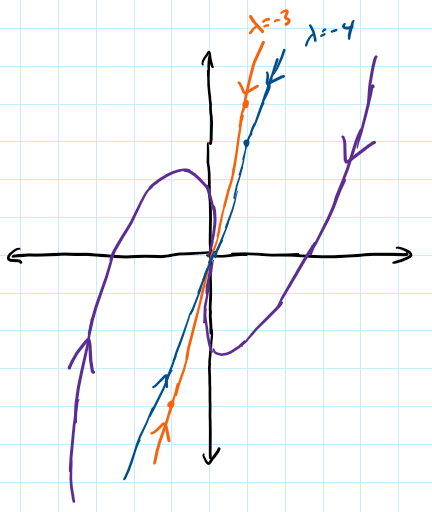
\includegraphics[height=1.5in]{Images/phaseportrait_n7_1_n12_0_sketch.png}}\hfill\hfill
%}%

\begin{exercise}%
    Find the general solution of the system
    \begin{equation*}
        {\vec{x}}' = 
        \begin{bmatrix} 
            -13 & -12 \\ 
            9 & 8 
        \end{bmatrix} \vec{x}
    \end{equation*}
    and draw a sketch for the phase portrait.\\
    $\vec{x}(t) = C_1 \left[\begin{smallmatrix} \answer{-4} \\ 3 \end{smallmatrix}\right]e^{-4t} + C_2 \left[\begin{smallmatrix} 1 \\ \answer{-1} \end{smallmatrix}\right] e^{-t}$
\end{exercise}
%\exsol{%
%$\vec{x}(t) = C_1 \left[\begin{smallmatrix} -4 \\ 3 \end{smallmatrix}\right]e^{-4t} + C_2 \left[\begin{smallmatrix} 1 \\ -1 \end{smallmatrix}\right] e^{-t}$ \hfill
%\raisebox{-0.5\height}{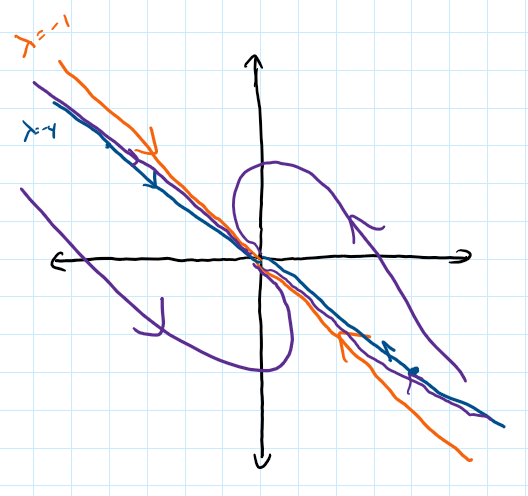
\includegraphics[height=1.5in]{Images/phaseportrait_n13_n12_9_8_sketch.png}}\hfill\hfill
%}%

\begin{exercise}%
    Find the general solution of the system
    \begin{equation*}
        {\vec{x}}' = 
        \begin{bmatrix} 
            -2 & -6 & 0 \\ 
            4 & 8 & 0 \\ 
            -4 & -7 & 3 
        \end{bmatrix} \vec{x}.
    \end{equation*}
    $\vec{x}(t) = C_1 \left[\begin{smallmatrix} \answer{0} \\ 0 \\ \answer{1} \end{smallmatrix}\right]e^{3t} + C_2 \left[\begin{smallmatrix} \answer{-1} \\ \answer{1} \\ -3 \end{smallmatrix}\right] e^{4t} + C_3 \left[\begin{smallmatrix} 3 \\ \answer{-2} \\ \answer{-2} \end{smallmatrix}\right] e^{2t}$
\end{exercise}
%\exsol{%
%$\vec{x}(t) = C_1 \left[\begin{smallmatrix} 0 \\ 0 \\ 1 \end{smallmatrix}\right]e^{3t} + C_2 \left[\begin{smallmatrix} -1 \\ 1 \\ -3 \end{smallmatrix}\right] e^{4t} + C_3 \left[\begin{smallmatrix} 3 \\ -2 \\ -2 \end{smallmatrix}\right] e^{2t}$
%}%

\begin{exercise}%
    Find the general solution of the system
    \begin{equation*}
        {\vec{x}}' = 
        \begin{bmatrix} 
            -6 & 2 & 4 \\ 
            -2 & -1 & 4 \\ 
            -2 & 1 & 0 
        \end{bmatrix} \vec{x}.
    \end{equation*}
    $\vec{x}(t) = C_1 \left[\begin{smallmatrix} \answer{2} \\ \answer{0} \\ 1 \end{smallmatrix}\right]e^{-4t} + C_2 \left[\begin{smallmatrix} 2 \\ \answer{3} \\ \answer{1} \end{smallmatrix}\right] e^{-t} + C_3 \left[\begin{smallmatrix} \answer{1} \\ 2 \\ \answer{0} \end{smallmatrix}\right] e^{-2t}$
\end{exercise}
%\exsol{%
%$\vec{x}(t) = C_1 \left[\begin{smallmatrix} 2 \\ 0 \\ 1 \end{smallmatrix}\right]e^{-4t} + C_2 \left[\begin{smallmatrix} 2 \\ 3 \\ 1 \end{smallmatrix}\right] e^{-t} + C_3 \left[\begin{smallmatrix} 1 \\ 2 \\ 0 \end{smallmatrix}\right] e^{-2t}$
%}%

\begin{exercise}
    Solve the initial value problem
    \[ 
        {\vec{x}}' = 
        \begin{bmatrix} 
            -3 & 0 \\ 
            3 & -4 
        \end{bmatrix} 
        \vec{x} \qquad \vec{x}(0) = 
        \begin{bmatrix} 
            -1 \\ 
            2 
        \end{bmatrix}. 
    \]
    $\vec{x}(t) = -\left[\begin{smallmatrix} \answer{1} \\ 3 \end{smallmatrix}\right]e^{-3t} + 5\left[\begin{smallmatrix} \answer{0} \\ 1 \end{smallmatrix}\right]e^{-4t}$
\end{exercise}
%\comboSol
%{%
%$\vec{x}(t) = -\left[\begin{smallmatrix} 1 \\ 3 \end{smallmatrix}\right]e^{-3t} + 5\left[\begin{smallmatrix} 0 \\ 1 \end{smallmatrix}\right]e^{-4t}$
%}

\begin{exercise}
    Solve the initial value problem
    \[ 
        {\vec{x}}' = 
        \begin{bmatrix} 
            1 & -3 \\ 
            2 & 6 
        \end{bmatrix} 
        \vec{x} \qquad \vec{x}(0) = 
        \begin{bmatrix} 
            1 \\ 
            1 
        \end{bmatrix}. 
    \]
    $\vec{x}(t) = -5\left[\begin{smallmatrix} \answer{1} \\ -1 \end{smallmatrix}\right]e^{4t} + 2\left[\begin{smallmatrix} 3 \\ \answer{-2} \end{smallmatrix}\right]e^{3t}$
\end{exercise}
%\comboSol
%{%
%$\vec{x}(t) = -5\left[\begin{smallmatrix} 1 \\ -1 \end{smallmatrix}\right]e^{4t} + 2\left[\begin{smallmatrix} 3 \\ -2 \end{smallmatrix}\right]e^{3t}$
%}

\begin{exercise}
    Solve the initial value problem
    \[ 
        {\vec{x}}' = 
        \begin{bmatrix} 
            7 & 4 & 0 \\ 
            -8 & -5 & 0 \\ 
            17 & 7 & -2 
        \end{bmatrix} 
        \vec{x} \qquad \vec{x}(0) = 
        \begin{bmatrix} 
            -3 \\ 
            2 \\ 
            2 
        \end{bmatrix}. 
    \]
    $\vec{x}(t) = \left[\begin{smallmatrix} \answer{1} \\ \answer{-2} \\ 3 \end{smallmatrix}\right]e^{-t} + 7\left[\begin{smallmatrix} 0 \\ \answer{0} \\ \answer{1} \end{smallmatrix}\right]e^{-2t} - 4\left[\begin{smallmatrix} \answer{1} \\ -1 \\ \answer{2} \end{smallmatrix}\right]e^{3t}$
\end{exercise}
%\comboSol
%{%
%$\vec{x}(t) = \left[\begin{smallmatrix} 1 \\ -2 \\ 3 \end{smallmatrix}\right]e^{-t} + 7\left[\begin{smallmatrix} 0 \\ 0 \\ 1 \end{smallmatrix}\right]e^{-2t} - 4\left[\begin{smallmatrix} 1 \\ -1 \\ 2 \end{smallmatrix}\right]e^{3t}$
%}


\end{document}